%-*- coding:utf-8 -*-

\documentclass[10pt,dvipdfmx]{beamer}
\usepackage{tutorial}

\title{計算機実験II (L8) --- 最適化問題(2)}
\date{2021/12/24}

\begin{document}

\begin{frame}
  \titlepage
  \tableofcontents
\end{frame}

\section{最適化問題}

\begin{frame}[t,fragile]{最適化問題}
  \begin{itemize}
    %\setlength{\itemsep}{1em}
  \item 目的関数$f(x)$の最小値(あるいは最大値)とその場所を求めたい
  \item どういう問題を解くのに使えるか?
    \begin{itemize}
    \item 変分原理が成り立つ問題: 最小作用の原理、最小エネルギーの原理$\cdots$
    \item コスト関数が定義できる問題: 最小二乗法(線形回帰、非線形回帰)、(連立)方程式、常/偏微分方程式、機械学習$\cdots$
    \end{itemize}
  \item ほぼ全ての問題は、コスト関数をうまく定義することで最適化問題に書き換えることができる
    \begin{itemize}
    \item (一般に)最適化問題として解くのは最終手段
    \item それぞれの問題に特化したより良い方法があるときはそちらを使う
    \end{itemize}
  \end{itemize}
\end{frame}

\begin{frame}[t,fragile]{様々な最適化手法}
  \begin{itemize}
    %\setlength{\itemsep}{1em}
  \item 最適化問題の種類
    \begin{itemize}
    \item 連続最適化問題 $\Leftarrow$ 目的関数が凸ではない場合、難しい
    \item 離散最適化(組み合せ最適化)問題 $\Leftarrow$ さらに難しい
    \end{itemize}
  \item 真の(大局的な)最小値(最大値)を求めるのは難しい
  \item 一般的には極値を求めることしかできない
  \item 多次元では極小を囲い込むことができない
  \item 導関数を使う方法: ニュートン法、準ニュートン法、最急降下法、勾配降下法、共役勾配法$\cdots$
  \item 使わない方法: 囲い込み法、Nelder-Meadの滑降シンプレックス法、シミュレーテッドアニーリング、量子アニーリング$\cdots$
  \item 目的関数・導関数の評価回数と収束までの反復回数のトレードオフ
  \end{itemize}
\end{frame}


\section{勾配の計算}

\begin{frame}[t,fragile]{数値微分(差分)}
  \begin{itemize}
    \setlength{\itemsep}{1em}
  \item 関数のテイラー展開
    \[
    f(x+h) = f(x) + h f'(x) + h^2 f''(x)/2 + h^3 f'''(x)/6 + \cdots
    \]
  \item 数値微分の最低次近似(前進差分)
    \[
    f_1(x,h) \equiv \frac{f(x+h)-f(x)}{h} = f'(x) + h f''(x)/2 + O(h^2)
    \]
  \item より高次の近似(中心差分)
    \[
    f_2(x,h) \equiv \frac{f(x+h)-f(x-h)}{2h} = f'(x) + h^2 f'''(x)/6 + O(h^3)
    \]
  \item 刻み$h$を小さくすると打ち切り誤差は減少するが、小さすぎると今度は桁落ちが大きくなる
  \end{itemize}
\end{frame}

% \begin{frame}[t,fragile]{差分の一般式}
  \begin{itemize}
    %\setlength{\itemsep}{1em}
  \item 関数のテイラー展開: $\displaystyle f(x+h) = \sum_{k} \frac{h^k}{k!} f^{(k)}(x)$
  \item $f^{(m)}(x)$を$n$個の$f(x+h_j)$の線形結合で表す($n \ge m+1$)
    \begin{align*}
      f^{(m)}(x) &\approx \sum_j a_j f(x+h_j) = \sum_j a_j \sum_{k} \frac{h_j^k}{k!} f^{(k)}(x) \\
      & = \sum_{k} C_k f^{(k)}(x) \qquad (C_k \equiv \sum_j a_j \frac{h_j^k}{k!})
    \end{align*}
  \item $C_k = \delta_{k,m}$ ($k = 0 \cdots n-1$)となるように$a_0 \cdots a_{n-1}$を決める
  \item 行列$\displaystyle G_{kj} = \frac{h_j^k}{k!}$と列ベクトル$a_j$と$b_k = \delta_{k,m}$を導入すると、条件式は$G a = b$と書ける (連立一次方程式)
  \end{itemize}
\end{frame}

\begin{frame}[t,fragile]{複素差分}
  \begin{itemize}
    %\setlength{\itemsep}{1em}
  \item 虚軸方向のテイラー展開を考える
    \[
    f(x+ih) = f(x) + ihf'(x) - h^2 f''(x)/2  - ih^3 f'''(x)/6 + \cdots
    \]
  \item テイラー展開の虚部を取ることで微分が求まる
    \[
    f'(x) = \frac{\mathrm{Im} (f(x+ih))}{h} + O(h^2)
    \]
  \item 引き算がないので桁落ちに強い
  \item 関数の値が複素数に対して正しく計算される必要がある
  \end{itemize}
\end{frame}

\begin{frame}[t,fragile]{前進差分・中心差分・複素差分}
  \begin{itemize}
    %\setlength{\itemsep}{1em}
  \item 精度の比較: $\frac{d}{dx} \sin(x^2) |_{x=\pi/2}$
    \begin{center}
      \resizebox{.75\textwidth}{!}{\includegraphics{image/diff.pdf}}
    \end{center}
  \end{itemize}
\end{frame}

\begin{frame}[t,fragile]{勾配の計算}
  \begin{itemize}
    %\setlength{\itemsep}{1em}
  \item $f(x_1,x_2,\cdots,x_d)$ の勾配
    \[
      \nabla f = \Large( \frac{\partial f}{\partial x_1}, \frac{\partial f}{\partial x_2}, \cdots, \frac{\partial f}{\partial x_d} \Large)
    \]
  \item 差分による計算
    \begin{itemize}
      \item 関数$f$の値を最低でも$2d$回評価する必要がある
      \item 方向によって適切な$h$の値は異なる → 関数評価の回数はさらに増加
    \end{itemize}
  \item 記号微分
    \begin{itemize}
      \item 数式処理(MATLAB, Mathematica等)により勾配の表式を計算
      \item $f$が複雑になると勾配の表式が長大に
      \item 勾配の値を評価するコストも大きくなる
    \end{itemize}
  \item 自動微分(automatic differentiation)
    \begin{itemize}
      \item 関数fの値の評価に必要なコストの定数倍の手間で勾配を評価可能
      \item ハイパーパラメータ$h$が存在しない
    \end{itemize}
  \end{itemize}
\end{frame}

\begin{frame}[t,fragile]{計算グラフ}
  \begin{itemize}
    %\setlength{\itemsep}{1em}
  \item 任意の関数の計算過程は、入力値と基本演算からなる計算グラフ(computation graph)で表現できる

    例: $\displaystyle f(x_1,x_2,x_3) = \frac{(x_1 - \exp(x_2)) x_3 \exp(x_2)}{x_3 \exp(x_2) + 1}$
    \begin{center}
      \resizebox{.45\textwidth}{!}{\includegraphics{image/compgraph.pdf}}
    \end{center}
    \vspace*{-2em} \hfill {\footnotesize [伊理・久保田(1991)]}
  \end{itemize}
\end{frame}

\begin{frame}[t,fragile]{関数値の評価}
  \begin{itemize}
    %\setlength{\itemsep}{1em}
  \item $\displaystyle f(x_1,x_2,x_3) = \frac{(x_1 - \exp(x_2)) x_3 \exp(x_2)}{x_3 \exp(x_2) + 1}$
  \item $(x_1,x_2,x_3)=(2,0,1)$における$f(x_1,x_2,x_3)$の値の評価
    \begin{itemize}
    \item $x_1 \leftarrow 2$
    \item $x_2 \leftarrow 0$
    \item $x_3 \leftarrow 1$
    \item $v_1 \leftarrow \exp(x_2) = 1$
    \item $v_2 \leftarrow x_1 - v_1 = 1$
    \item $v_3 \leftarrow v_1 \times x_3 = 1$
    \item $v_4 \leftarrow v_2 \times v_3 = 1$
    \item $v_5 \leftarrow v_3 + 1 = 2$
    \item $f \leftarrow v_4 / v_5 = 1/2$
    \end{itemize}
    \vspace*{-7em} \hfill \resizebox{.3\textwidth}{!}{\includegraphics{image/compgraph.pdf}}
  \end{itemize}
\end{frame}

\begin{frame}[t,fragile]{合成関数の微分}
  \begin{itemize}
    %\setlength{\itemsep}{1em}
  \item $f(x_1,x_2,x_3)$の$x_2$に関する偏導関数の計算
  \item 連鎖律(chain rule)
    \[
      \frac{\partial f}{\partial x_2} = \frac{\partial f}{\partial v_4} \frac{\partial v_4}{\partial x_2} + \frac{\partial f}{\partial v_5} \frac{\partial v_5}{\partial x_2} = \frac{\partial f}{\partial v_4} \frac{\partial v_4}{\partial v_2} \frac{\partial v_2}{\partial x_2} + \frac{\partial f}{\partial v_4} \frac{\partial v_4}{\partial v_3} \frac{\partial v_3}{\partial x_1} + \cdots
    \]
    \begin{itemize}
    \item $\displaystyle \frac{\partial f}{\partial x_2}$ は計算経路(全部で7つ)の和で書ける
    \end{itemize}
  \item 経路の例
    \begin{itemize}
    \item $\displaystyle \frac{\partial f}{\partial v_4} \frac{\partial v_4}{\partial v_2} \frac{\partial v_2}{\partial v_1} \frac{\partial v_1}{\partial x_2} \frac{\partial x_2}{\partial x_2} $
    \item $\displaystyle \frac{\partial f}{\partial v_5} \frac{\partial v_5}{\partial v_3} \frac{\partial v_3}{\partial x_3} \frac{\partial x_3}{\partial x_2} (=0)$
    \end{itemize}
    \vspace*{-7em} \hfill \resizebox{.3\textwidth}{!}{\includegraphics{image/compgraph.pdf}}
  \end{itemize}
\end{frame}

\begin{frame}[t,fragile]{自動微分}
  \begin{itemize}
    %\setlength{\itemsep}{1em}
  \item 前進モード(Forward mode)・ボトムアップ型(Bottom-up)計算
  \item 計算グラフを下から順番に計算していく
    \begin{itemize}
    \item $\displaystyle \frac{\partial x_1}{\partial x_2} = 0$,
      $\displaystyle \frac{\partial x_2}{\partial x_2} = 1$,
      $\displaystyle \frac{\partial x_3}{\partial x_2} = 0$,
      $\displaystyle \frac{\partial 1}{\partial x_2} = 0$
    \item $\displaystyle \frac{\partial v_1}{\partial x_2} = \frac{\partial}{\partial x_2} \exp(x_2) = \exp(0) = 1$
    \item $\displaystyle \frac{\partial v_2}{\partial x_2} = \frac{\partial x_1}{\partial x_2} - \frac{\partial v_1}{\partial x_2} = 0-1 = -1$
    \item $\displaystyle \frac{\partial v_3}{\partial x_2} = \frac{\partial v_1}{\partial x_2} x_3 +  v_1 \frac{\partial x_3}{\partial x_2} = 1 \times 1 + 1 \times 0 = 1$
    \item $\displaystyle \frac{\partial v_4}{\partial x_2} = \frac{\partial v_2}{\partial x_2} v_3 +  v_2  \frac{\partial v_3}{\partial x_2} = (-1) \times 1 + 1 \times 1 = 0$
    \item $\displaystyle \frac{\partial v_5}{\partial x_2} = \frac{\partial v_3}{\partial x_2} +   \frac{\partial 1}{\partial x_2} = 1 + 0 = 1$
    \item $\displaystyle \frac{\partial f}{\partial x_2} = \frac{\partial}{\partial x_2} \frac{v_4}{v_5} = \frac{\frac{\partial v_4}{\partial x_2} v_5 - v_4 \frac{\partial v_5}{\partial x_2}}{(v_5)^2} = \frac{0 \times 2 - 1 \times 1}{2^2} = -1/4$
    \end{itemize}
    \vspace*{-16em} \hfill \resizebox{.3\textwidth}{!}{\includegraphics{image/compgraph.pdf}}
  \end{itemize}
\end{frame}

\begin{frame}[t,fragile]{テイラー展開による前進モードの計算}
  \begin{itemize}
    %\setlength{\itemsep}{1em}
  \item $x_2 = 0 + \epsilon$, $x_1 = 2$, $x_3 = 1$と表す
  \item 途中の計算を $\epsilon$ の1次まで保存しながら計算
    \begin{itemize}
    \item $v_1 \leftarrow \exp(x_2) = \exp(0 + \epsilon) \approx 1 + \epsilon$
    \item $v_2 \leftarrow x_1 - v_1 = 2 - (1 + \epsilon) = 1 - \epsilon$
    \item $v_3 \leftarrow v_1 \times x_3 = (1 + \epsilon) \times 1 = 1 + \epsilon$
    \item $v_4 \leftarrow v_2 \times v_3 = (1 - \epsilon) \times (1 + \epsilon) \approx 1$
    \item $v_5 \leftarrow v_3 + 1 = (1 + \epsilon) + 1 = 2 + \epsilon$
    \item $f \leftarrow v_4 / v_5 = 1 / (2 + \epsilon) \approx \frac{1}{2} - \frac{1}{4} \epsilon$
    \end{itemize}
  \item $\epsilon$ の係数が微分の値
  \item それぞれの基本演算に対するテイラー展開係数の計算式を用意しておけばよい \ 例)
    \begin{itemize}
    \item $(a + b \epsilon) \times (c + d \epsilon) \approx ac + (ad + bc) \epsilon$
    \item $\exp(a+b\epsilon) \approx \exp(a) + \exp(a) b \epsilon$
    \end{itemize}
  \item 1つの独立変数に関する偏導関数の計算は、関数値$f$の計算コストと同じオーダー → 勾配を計算するにはその$n$倍の計算量が必要

    \vspace*{-17em} \hfill \resizebox{.3\textwidth}{!}{\includegraphics{image/compgraph.pdf}}
  \end{itemize}
\end{frame}

\begin{frame}[t,fragile]{自動微分(後退モード)}
  \begin{itemize}
    %\setlength{\itemsep}{1em}
  \item 後退モード(Backward mode)・トップダウン型(Top-down)計算
  \item まず、下から順に $v_1, v_2, \cdots$ の値、および各基本演算における微分係数をもとめておく
    \begin{itemize}
    \item $v_1 \leftarrow \exp(x_2) = 1$, $d_{v_1,x_2} \leftarrow \frac{\partial v_1}{\partial x_2} = \exp(x_2) = 1$
    \item $v_2 \leftarrow x_1 - v_1 = 1$, $d_{v_2,x_1} \leftarrow \frac{\partial v_2}{\partial x_1} = 1$, $d_{v_2,v_1} \leftarrow \frac{\partial v_2}{\partial v_1} = -v_1 = -1$,
    \item $v_3 \leftarrow v_1 \times x_3 = 1$, $d_{v_3,v_1} \leftarrow \frac{\partial v_3}{\partial v_1} = x_3 = 1$, $d_{v_3,x_3} \leftarrow \frac{\partial v_3}{\partial x_3} = v_1 = 1$
    \item $v_4 \leftarrow v_2 \times v_3 = 1$
    \item $d_{v_4,v_2} \leftarrow \frac{\partial v_4}{\partial v_2} = v_3 = 1$
    \item $d_{v_4,v_3} \leftarrow \frac{\partial v_4}{\partial v_3} = v_2 = 1$
    \item $v_5 \leftarrow v_3 + 1 = 2$
    \item $d_{v_5,v_3} \leftarrow \frac{\partial v_5}{\partial v_3} = 1$
    \item $f \leftarrow v_4 / v_5 = 1/2$
    \item $d_{f,v_4} \leftarrow \frac{\partial f}{\partial v_4} = \frac{1}{v_5} = \frac{1}{2}$
    \item $d_{f,v_5} \leftarrow \frac{\partial f}{\partial v_5} = -\frac{v_4}{(v_5)^2} = -\frac{1}{4}$
    \end{itemize}
    \vspace*{-9em} \hfill \resizebox{.3\textwidth}{!}{\includegraphics{image/compgraph.pdf}}
  \end{itemize}
\end{frame}

\begin{frame}[t,fragile]{自動微分(後退モード)}
  \begin{itemize}
    %\setlength{\itemsep}{1em}
  \item 次に上から順番に連鎖律を適用
    \begin{itemize}
    \item $\frac{\partial f}{\partial v_5} = d_{f,v_5} = -\frac{1}{4}$
    \item $\frac{\partial f}{\partial v_4} = d_{f,v_4} = \frac{1}{2}$
    \item $\frac{\partial f}{\partial v_3} = \frac{\partial f}{\partial v_4} \frac{\partial v_4}{\partial v_3} +  \frac{\partial f}{\partial v_5} \frac{\partial v_5}{\partial v_3}  = d_{f,v_4} d_{v_4,v_3} + d_{f,v_5} d_{v_5,v_3} = \frac{1}{2} \cdot 1 -\frac{1}{4} \cdot 1 = \frac{1}{4}$
    \item $\frac{\partial f}{\partial v_2} = \frac{\partial f}{\partial v_4} \frac{\partial v_4}{\partial v_2} = d_{f,v_4} d_{v_4,v_2} =  \frac{1}{2} \cdot 1 = \frac{1}{2}$
    \item $\frac{\partial f}{\partial v_1} = \frac{\partial f}{\partial v_2} \frac{\partial v_2}{\partial v_1} +  \frac{\partial f}{\partial v_3} \frac{\partial v_3}{\partial v_1} = d_{f,v_2} d_{v_2,v_1} + d_{f,v_3} d_{v_3,v_1} = \frac{1}{2} \cdot (-1) + \frac{1}{4} \cdot 1 = -\frac{1}{4}$
    \item $\frac{\partial f}{\partial x_3} = \frac{\partial f}{\partial v_3} \frac{\partial v_3}{\partial x_3} = \frac{1}{4} \cdot 1 = \frac{1}{4}$
    \item $\frac{\partial f}{\partial x_2} = \frac{\partial f}{\partial v_1} \frac{\partial v_1}{\partial x_2} = -\frac{1}{4} \cdot 1 = -\frac{1}{4}$
    \item $\frac{\partial f}{\partial x_1} = \frac{\partial f}{\partial v_2} \frac{\partial v_2}{\partial x_1} = d_{f,v_2} d_{v_2,x_1} = \frac{1}{2} \cdot 1 = \frac{1}{2}$
    \end{itemize}
  \item 計算の過程で、全ての独立・中間変数に関する偏導関数が自動的に求まる
  \item 計算量は$f$の値を計算するコストの定数倍

    % \vspace*{-10em} \hfill \resizebox{.3\textwidth}{!}{\includegraphics{image/compgraph.pdf}}
  \end{itemize}
\end{frame}

\begin{frame}[t,fragile]{自動微分}
  \begin{itemize}
    %\setlength{\itemsep}{1em}
  \item 独立変数の次元が$n$, 関数値の次元が$m$のとき
    \begin{itemize}
    \item $n \ll m$: 前進モードが効率的
    \item $n \gg m$: 後退モードが効率的
    \end{itemize}
  \item $m=1$のとき: $f=f(x_1,x_2, \cdots x_n)$
    \begin{itemize}
    \item ある方向$\mathbf{p}$に沿った微分 → 前進モードにより効率的に計算可
    \item ヘッセ行列$\displaystyle H_{ij} = \frac{\partial^2 f}{\partial x_i \partial x_j}$とベクトル$\mathbf{p}$の積 → 後退モードにより効率的に計算可
    \end{itemize}
  \item 深層学習(ニューラルネットワーク)における最適化
    \begin{itemize}
    \item バックプロパゲーションによる勾配の計算: 自動微分(後退モード)と等価
    \end{itemize}
  \end{itemize}
\end{frame}


\section{Nelder-Meadの滑降シンプレックス法}

\begin{frame}[t,fragile]{Nelder-Meadの滑降シンプレックス法}
  \begin{itemize}
    %\setlength{\itemsep}{1em}
  \item 関数値のみ。導関数の情報を必要としない
  \item プログラミングが簡単
  \item 収束は遅いが、安定に極小値が求まる
  \item $d+1$個の頂点からなる$d$次元の超多面体(シンプレックス)を変形しながら、極小値を探す
    \begin{itemize}
    \item 2次元: 三角形
    \item 3次元: 四面体
    \end{itemize}
  \item 別名「アメーバ法」
  \end{itemize}
\end{frame}

\begin{frame}[t,fragile]{Nelder-Meadの滑降シンプレックス法}
  \begin{itemize}
    %\setlength{\itemsep}{1em}
  \item $d+1$個の点$x_0,x_1,\cdots,x_d$は$f(x_0) \le f(x_1) \le \cdots \le f(x_d)$の順に並べられているとする
  \item 最大値を取る点$x_d$を除く$d$点の重心を$x_g$とする
  \item Nelder-Mead法では以下のステップを繰り返す
    \begin{itemize}
    \item $x_d$を$x_g$に関する対称な点$x_r$に移動(反射)
      \[
      x_r = x_g + (x_g - x_d)
      \]
    \item $f(x_r)$が$f(x_0)$よりも小さい場合、さらに先に進む(拡大)
      \[
      x_e = x_g + 2(x_r - x_g)
      \]
    \item $f(x_r)$が$f(x_{d-1})$よりもまだ大きい場合には、$x_d$を$x_g$に近づける(縮小)
      \[
      x_c = x_g + (x_d-x_g)/2
      \]
    \item $f(x_c)$が$f(x_d)$よりまだ大きい場合には、$x_0$以外の点を$x_0$に一様に近づける(収縮)
      \[
      x_i \leftarrow x_0 + (x_i-x_0)/2 \qquad (i=1 \cdots d)
      \]
    \end{itemize}
  \end{itemize}
\end{frame}

% -*- coding: utf-8 -*-

\begin{frame}[t,fragile]{Nelder-Meadの滑降シンプレックス法}
  \vspace*{-2em}
  \hspace*{1em}\resizebox{!}{1.0\textheight}{\includegraphics{image/neldermead.pdf}}

  \vspace*{-4em}
  \hspace*{18em}{\tiny\url{http://www.kniaz.net/software/RosNM.aspx}}
\end{frame}


\section{量子アニーリング (復習)}

\begin{frame}[t,fragile]{量子アニーリング}
  \begin{itemize}
    %\setlength{\itemsep}{1em}
  \item 離散最適化問題
    \[
    H = -J \sum_{i<j} \epsilon_{ij} \sigma_i^z \sigma_j^z
    \]
    の基底状態配位と基底状態エネルギーを求めたい
    \begin{center}
      \resizebox{0.6\textwidth}{!}{\includegraphics{image/spinglass.pdf}}
    \end{center}
  \end{itemize}
\end{frame}

\begin{frame}[t,fragile]{量子アニーリング}
  \begin{itemize}
    %\setlength{\itemsep}{1em}
  \item 横磁場を導入
    \[
    H = -J \sum_{i<j} \epsilon_{ij} \sigma_i^z \sigma_j^z - \Gamma \sum_i \sigma_i^x
    \]
  \item 古典極限 ($J=1$, $\Gamma=0$)
    \begin{itemize}
    \item 求めたい基底状態
    \end{itemize}
  \item 量子極限 ($J=0$, $\Gamma=1$)
    \begin{itemize}
    \item $2^N$個の全ての状態の重ね合わせ
    \end{itemize}
  \item 量子アニーリング
    \begin{itemize}
    \item $J+\Gamma=1$を保ったままで、$\Gamma=1$から$\Gamma=0$まで「ゆっくり」と減少させながら時間発展させる
      \[
      J = 1-\Gamma = t/T \qquad (0 \le t \le T)
      \]
    \item $T \rightarrow \infty$の極限で確率1で基底状態に収束
    \end{itemize}
  \end{itemize}
\end{frame}


\section{シミュレーテッドアニーリング}

\begin{frame}[t,fragile]{確率過程を用いた最適化}
  \begin{itemize}
    %\setlength{\itemsep}{1em}
  \item 最急降下法 (steepest decent)% {\footnotesize \href{https://github.com/todo-group/computer-experiments/blob/master/exercise/optimization/mc_steepest_descent_1d.c}{mc\_steepest\_descent\_1d.c}}
    \begin{itemize}
    \item 初期状態をランダムに定める
    \item 配位を少しだけ変化させる
    \item エネルギー(コスト関数)が小さくなるなら採択、大きくなるなら棄却 $\Rightarrow$ 絶対零度でのMetropolis法と等価
    \item 状態が変化しなくなるまでくり返す
    \item 問題点 : エネルギー極小状態にすぐに捕まってしまう
    \end{itemize}
  \item 徐冷法 (simulated annealing)% {\footnotesize \href{https://github.com/todo-group/computer-experiments/blob/master/exercise/optimization/simulated_annealing_1d.c}{simulated\_annealing\_1d.c}}
    \begin{itemize}
    \item いきなり温度を零にするのではなく少しずつ下げていく
    \item どれくらいゆっくり下げれば良いか?
      \[
      T(t) \ge cN / \log(t+2)
      \]
    \item 実際には適当なスケジューリングで温度を下げ、何回か繰り返して最も良い結果を採択
    \end{itemize}
  \end{itemize}
\end{frame}

\begin{frame}[t,fragile]{Metropolis法}
  \begin{itemize}
    \setlength{\itemsep}{1em}
  \item 現在の配位$x$から、試行配位(trial configuration) $x'$を$x - \Delta \sim x + \Delta$の一様分布より選ぶ
  \item 確率$\min \Big( 1, \frac{e^{-\beta V(x')}}{e^{-\beta V(x)}} \Big)$で$x'$を採択(accept)。棄却(reject)された場合にはもとの$x$のまま
  \item 物理量の測定 (reject された場合にもカウントする)
  \item 採択確率(acceptance probability)は、$\frac{e^{-\beta V(x')}}{e^{-\beta V(x)}+e^{-\beta V(x')}}$でもよい
  \item 例: \href{https://github.com/todo-group/computer-experiments/blob/master/exercise/monte_carlo/harmonic.c}{harmonic.c}
  \end{itemize}
\end{frame}

% -*- coding: utf-8 -*-

\begin{frame}[t,fragile]{最急降下法とシミュレーテッドアニーリング}
  \noindent\resizebox{0.45\textwidth}{!}{\includegraphics{image/potential.pdf}}

  \noindent\hspace*{.5em}\resizebox{0.43\textwidth}{!}{\includegraphics{image/boltzmann.pdf}}

  \vspace*{-17em}\hspace*{12.5em}\resizebox{0.6\textwidth}{!}{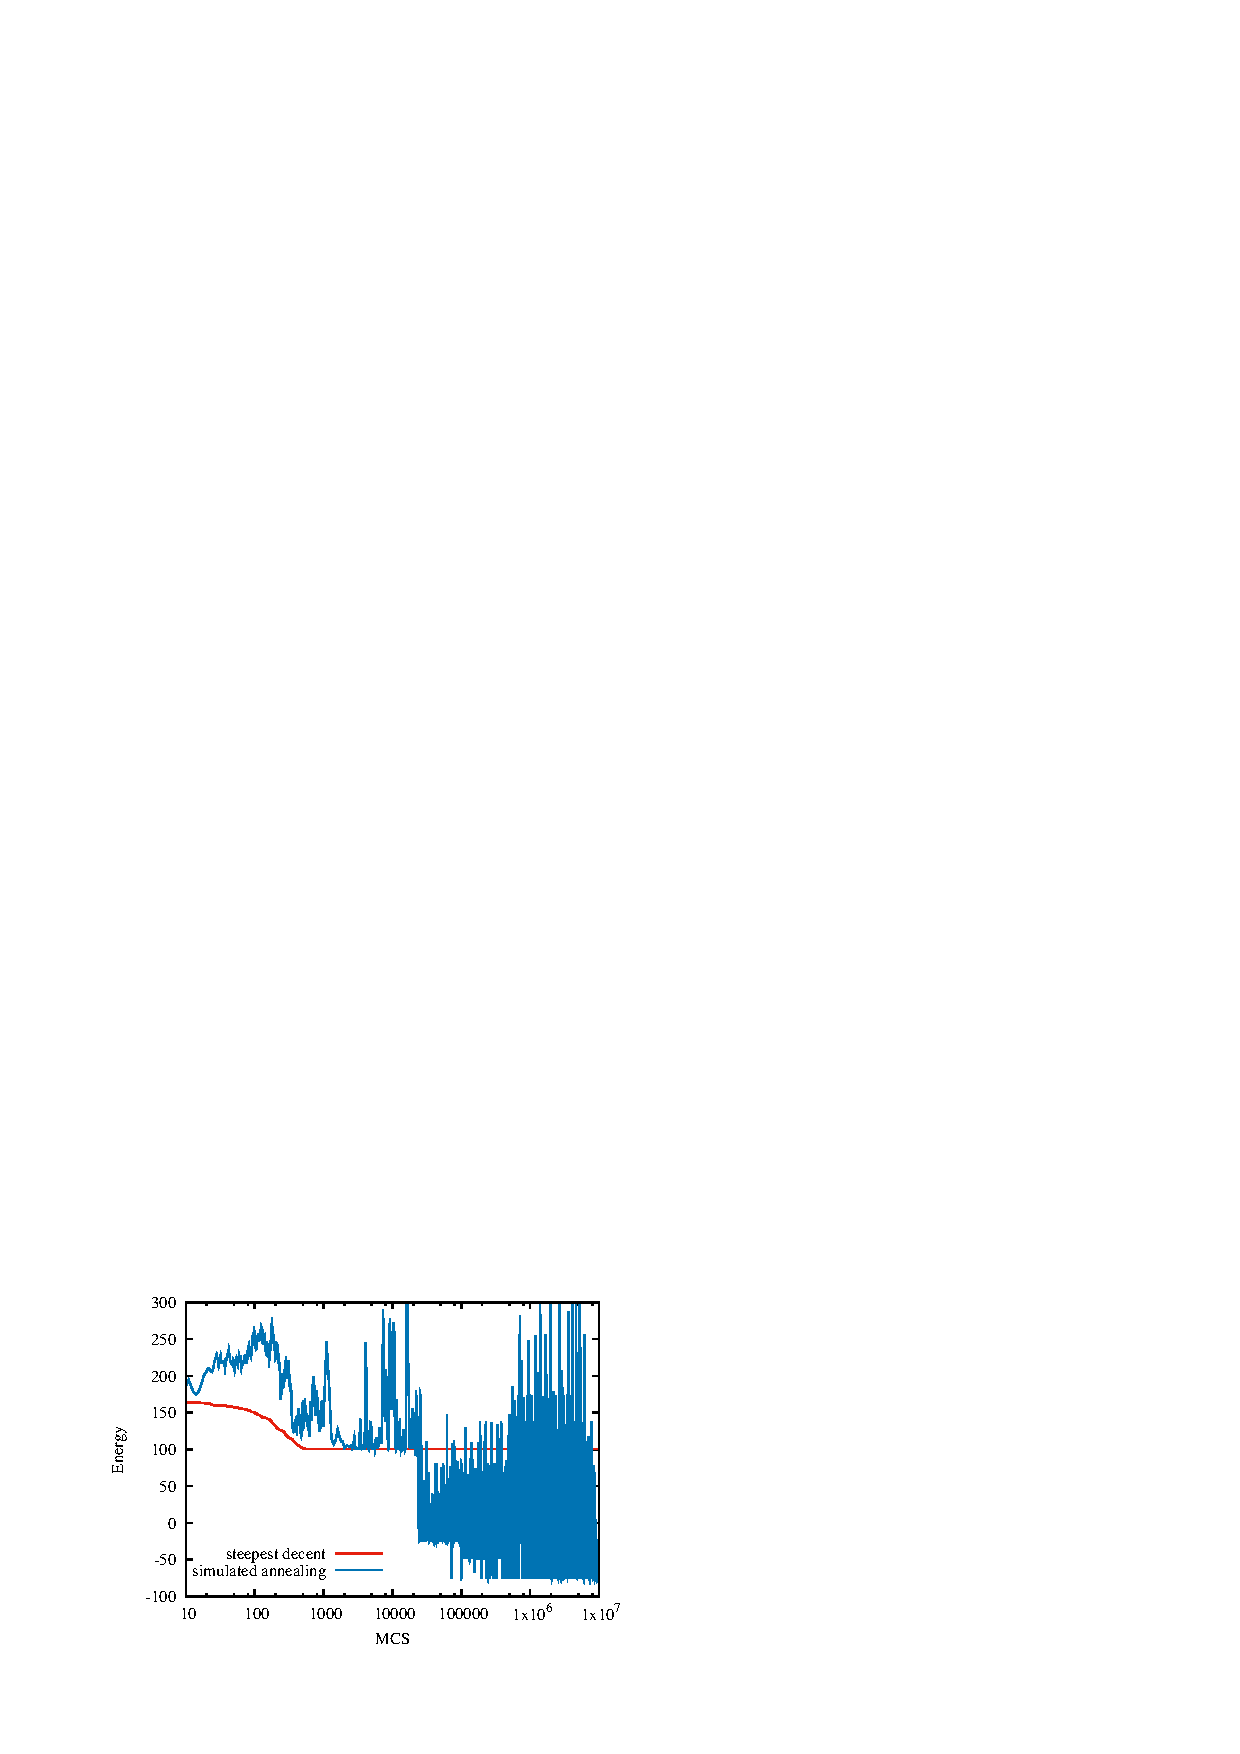
\includegraphics{image/energy.pdf}}

  \hspace*{17em}$T(t) = 100 - \frac{99}{10^7} t$
\end{frame}


\section{最適化手法の比較}

\begin{frame}[t,fragile]{例題 (二次元の最適化)}
  \begin{center}
    \resizebox{.9\textwidth}{!}{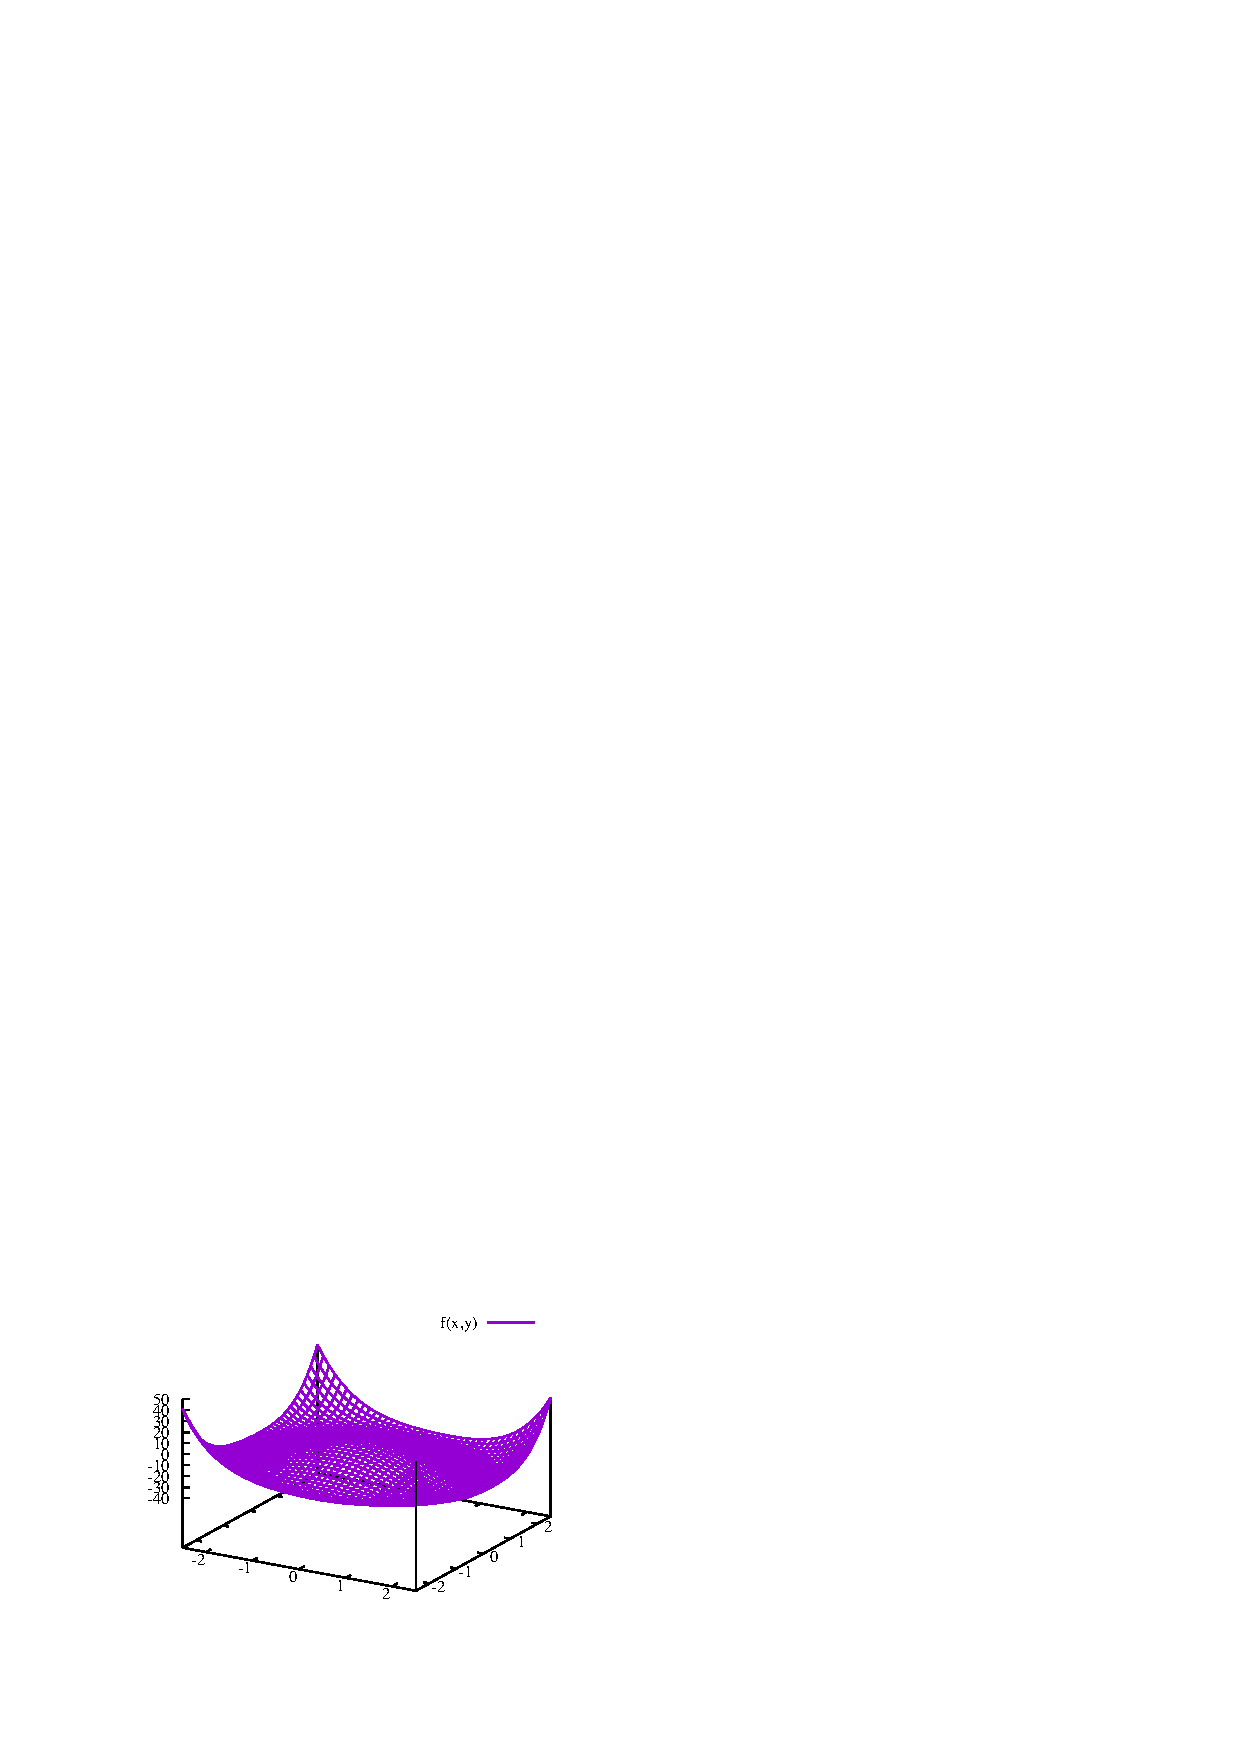
\includegraphics{image/func_2d.pdf}}
  \end{center}
\end{frame}

\begin{frame}[t,fragile]{様々な最適化手法の比較 (1/4)}
  \begin{center}
    \resizebox{.9\textwidth}{!}{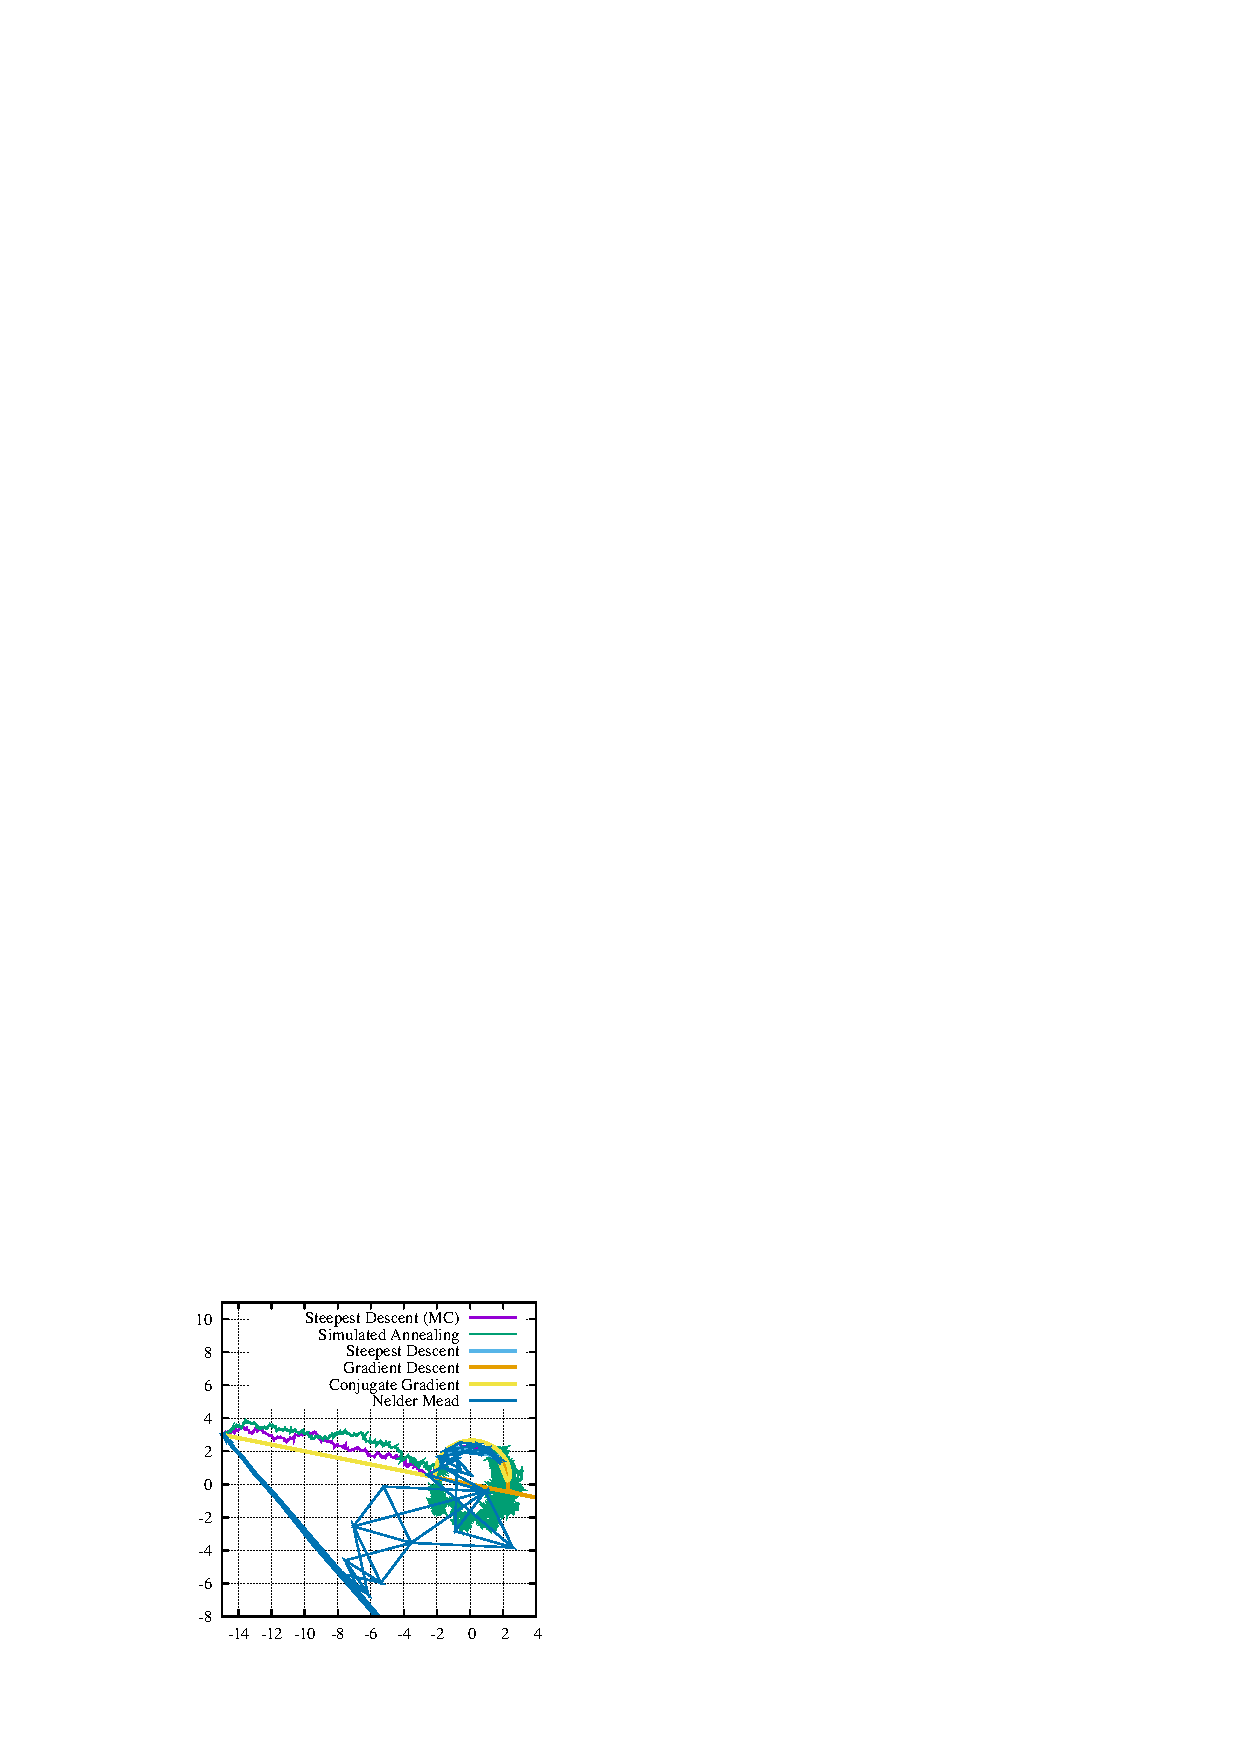
\includegraphics{image/optimization.pdf}}
  \end{center}
\end{frame}

\begin{frame}[t,fragile]{様々な最適化手法の比較 (2/4)}
  \begin{center}
    \resizebox{.9\textwidth}{!}{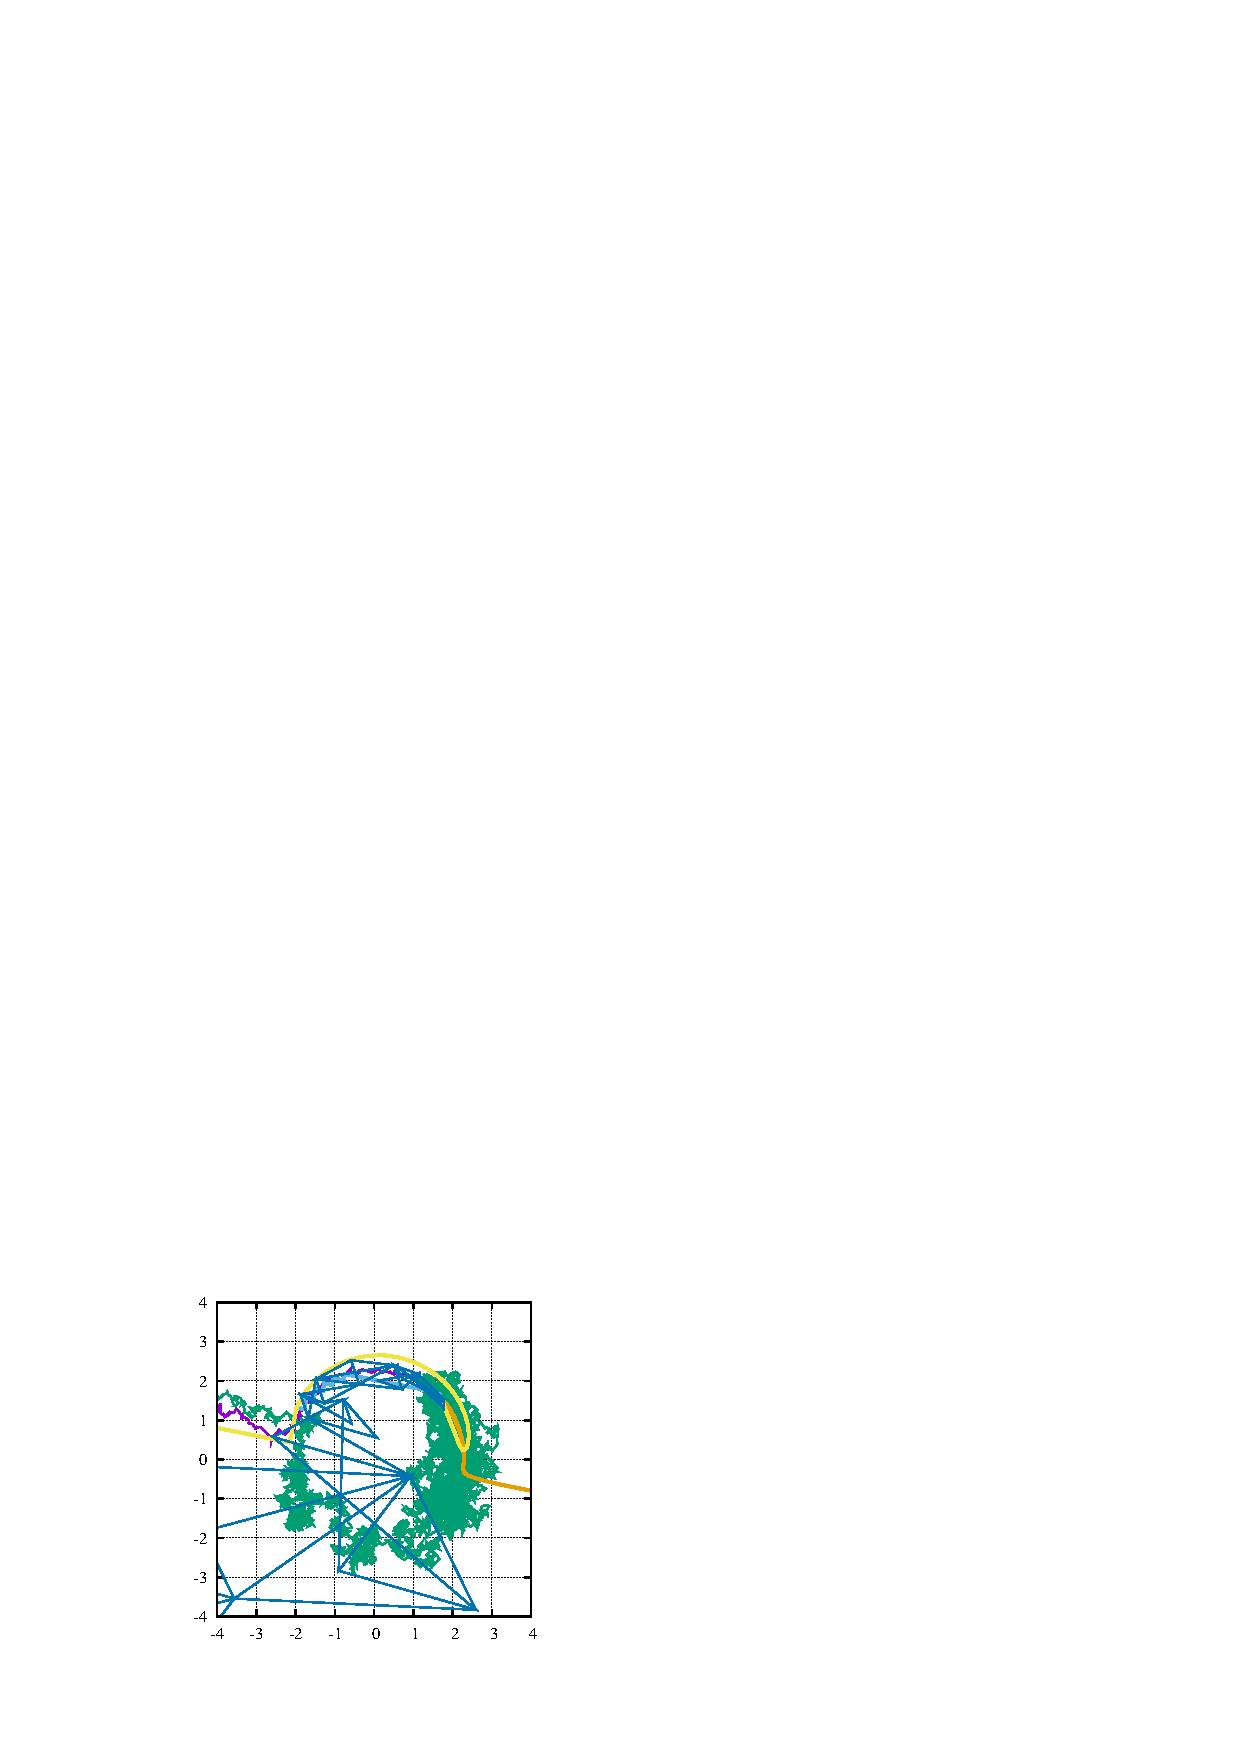
\includegraphics{image/optimization2.pdf}}
  \end{center}
\end{frame}

\begin{frame}[t,fragile]{様々な最適化手法の比較 (3/4)}
  \begin{center}
    \resizebox{.9\textwidth}{!}{\includegraphics{image/optimization3.pdf}}
  \end{center}
\end{frame}

\begin{frame}[t,fragile]{様々な最適化手法の比較 (4/4)}
  \begin{center}
    \resizebox{.9\textwidth}{!}{\includegraphics{image/optimization4.pdf}}
  \end{center}
\end{frame}

\begin{frame}[t,fragile]{真の解への近づき方}
  \begin{center}
    \resizebox{.9\textwidth}{!}{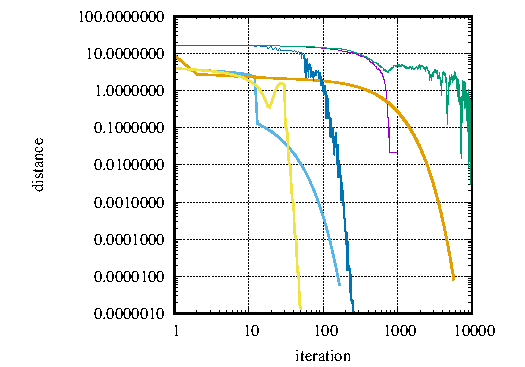
\includegraphics{image/convergence.pdf}}
  \end{center}
\end{frame}


\section{}

\begin{frame}[t,fragile]{計算機環境}
  \begin{itemize}
    %\setlength{\itemsep}{1em}
  \item 教育用計算機システム
  \item 知の物理学クラスタ(ai)
    \begin{itemize}
    \item 卒業まで利用可 (希望すれば大学院でも)
    \item バッチシステムを使えば、かなり大規模な計算も可能
    \end{itemize}
  \item 計算機利用・シミュレーションに関する質問は今後も歓迎 {\tt computer@phys.s.u-tokyo.ac.jp}
  \end{itemize}
\end{frame}

\begin{frame}[t]{講義日程 (予定)}
  \begin{itemize}
    % \setlength{\itemsep}{1em}
  \item 全8回 (金曜5限 16:50-18:35)
    \begin{itemize}
    \item 10月4日(金) 講義1: 多体系の統計力学とモンテカルロ法
    \item {\color{gray} 10月11日(金) 休講 (物理学教室コロキウム)}
    \item 10月18日(金) 実習1
    \item {\color{gray} 10月25日(金) 休講}
    \item 11月1日(金) 講義2: 偏微分方程式と多体系の量子力学
    \item 11月8日(金) 実習2
    \item {\color{gray} 11月15日(金) 休講}
    \item 11月29日(金) 講義3: 少数多体系・分子動力学
    \item 12月6日(金) 実習3
    \item {\color{gray} 12月13日(金) 休講 (物理学教室コロキウム)}
    \item {\color{gray} 12月20日(金) 休講 (ニュートン祭)}
    \item 12月27日(金) 講義4: 最適化問題
    \item 1月10日(金) 実習4
    \item {\color{gray} 1月24日(金) 休講 (物理学教室コロキウム)}
    \end{itemize}
  \end{itemize}
\end{frame}


\begin{frame}[t]{本日の課題}
  \begin{itemize}
    %\setlength{\itemsep}{1em}
  \item 授業評価アンケートに回答お願いします
  \item 実習
    \begin{itemize}
    \item 実習課題一覧\href{https://github.com/todo-group/ComputerExperiments/releases/tag/2021a-computer2}{exercise-2.pdf}から最適化(あるいは別の)課題を選び実習
    \end{itemize}
  \item 質問はSlackの「\# 8\_最適化」あるいは他の適当と思われるチャンネルで
  \item 本日24時までにITC-LMSのアンケート「第8回(12/24)作業レポート」に回答(出席のかわり)
    \begin{itemize}
    \item 1月7日のもくもく会は、アンケートで希望者がいる場合のみ実施
    \end{itemize}
  \item 「レポートNo.2」 (ITC-LMSを参照) 締切 2021/01/17(月)
  \end{itemize}
\end{frame}

\end{document}
